\documentclass[]{beamer}
% Class options include: notes, notesonly, handout, trans,
%                        hidesubsections, shadesubsections,
%                        inrow, blue, red, grey, brown

% Theme for beamer presentation.
\usepackage{beamerthemesplit,subfigure} 
\usepackage{subfigure}
% Other themes include: beamerthemebars, beamerthemelined, 
%                       beamerthemetree, beamerthemetreebars  

\title{Thermal Conductivity from \textit{ab initio} Phonon Properties}    % Enter your title between curly braces
\author{Samuel Huberman}                 % Enter your name between curly braces
\institute{ECE 1336}      % Enter your institute name between curly braces
\date{\today}                    % Enter the date or \today between curly braces

\begin{document}
\setbeamercolor{block title}{fg=blue}

% Creates title page of slide show using above information
\begin{frame}
  \titlepage
\end{frame}

\section[Outline]{}

% Creates table of contents slide incorporating
% all \section and \subsection commands
\begin{frame}
  \tableofcontents
\end{frame}


\section{Background and Experiment}
\begin{frame}
  \frametitle{Phonon Phenomena}   % Insert frame title between curly braces

  \begin{itemize}
  \item Joule Heating: Current carriers interact with atomic ions, transferring electrical energy to thermal energy.
  \item Superconductivity: Small phonon contribution to the photoemission kink in the copper oxide superconductors (Nature 2008)
  \item Entanglement: Entangling Macroscopic Diamonds at Room Temperature (Science 2011)
  \end{itemize} 
\end{frame}


\begin{frame}
  \frametitle{Experimental studies}   % Insert frame title between curly braces
\begin{figure}[ht]
\centering
\subfigure[Neutron Scattering]{
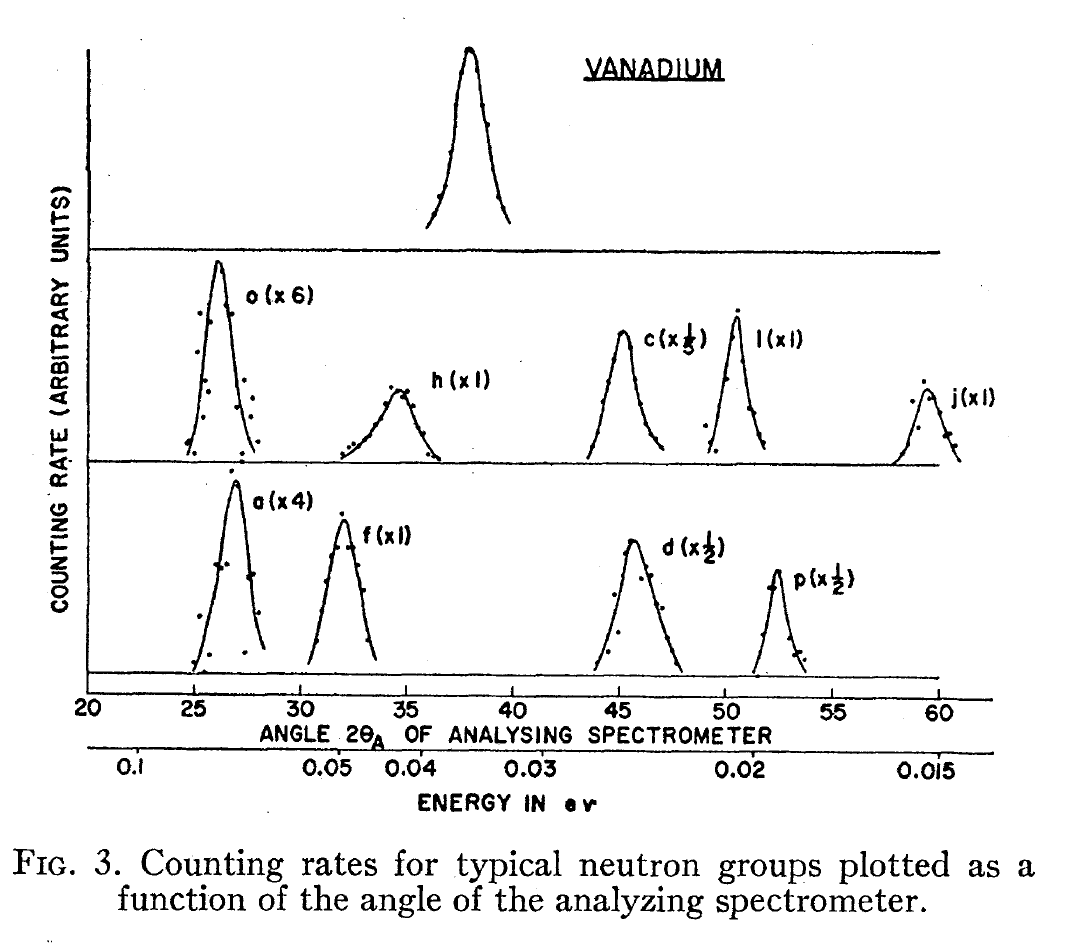
\includegraphics[scale=0.125]{neutron.png}
\label{fig:subfig1}
}
\subfigure[Raman Spectroscopy]{
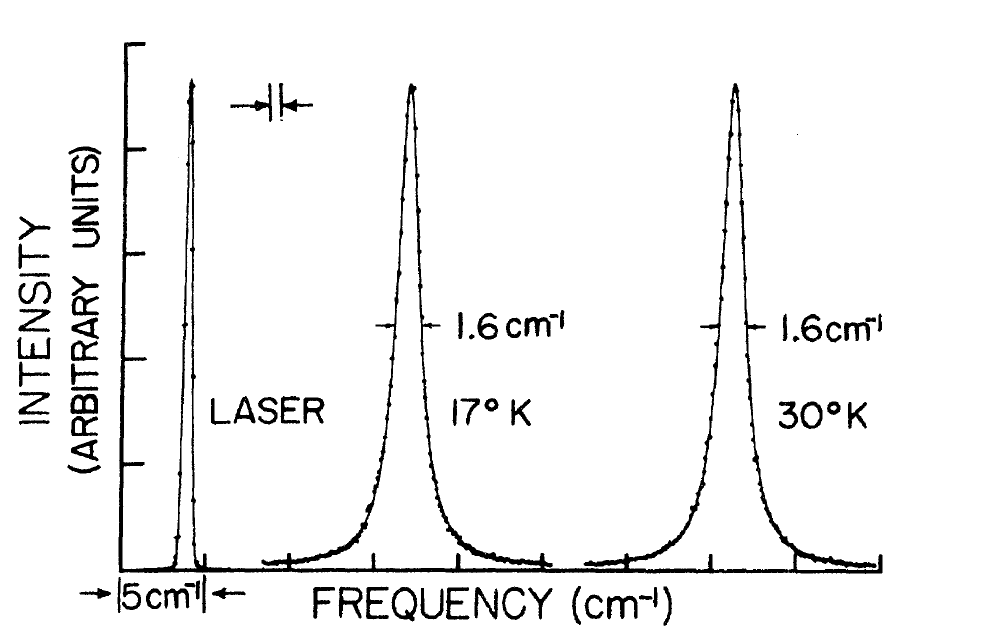
\includegraphics[scale=0.2]{raman.png}
\label{fig:subfig2}
}
\end{figure}
\end{frame}

\section{Theory and Modelling}

\begin{frame}
  \frametitle{Continuum approach}   % Insert frame title between curly braces

  \begin{itemize}
  \item Recall Fourier's Law of heat conduction:
	\begin{align*}
		q=-k\frac{\partial T}{\partial x}
	\end{align*}
  \item What happens when the length scales become comparable with MFP?
  \end{itemize}
\end{frame}

\begin{frame}
  \frametitle{Boltzmann Transport Equation}   % Insert frame title between curly braces

  \begin{itemize}
  \item ``Phonon gas'' picture:
\begin{align*}
	\frac{\partial f(\pmb{\kappa}, \nu)}{\partial t}+v_g(\pmb{\kappa}, \nu)\cdot\nabla f(\pmb{\kappa}, \nu)= [\frac{\partial f(\pmb{\kappa}, \nu)}{\partial t}]_{coll}
\end{align*}
  \item Under the relaxation time approximation:
\begin{align*}
	\frac{\partial f(\pmb{\kappa}, \nu)}{\partial t}+v_g(\pmb{\kappa}, \nu)\cdot\nabla f(\pmb{\kappa}, \nu)= \frac{f^{BE}(\pmb{\kappa}, \nu)-f(\pmb{\kappa}, \nu)}{\tau(\pmb{\kappa}, \nu)}
\end{align*}
  \item Thermal conductivity:
	\begin{align*}
		k(L)=\sum_\nu \sum_\kappa c_{ph}(\pmb{\kappa},\nu)v^2_g(\pmb{\kappa}, \nu)\tau(\pmb{\kappa}, \nu,L)
	\end{align*}
  \item We need phonon properties!
  \end{itemize}
\end{frame}

\begin{frame}
  \frametitle{Diatomic Chain}   % Insert frame title between curly braces
\begin{figure}[ht]
\centering
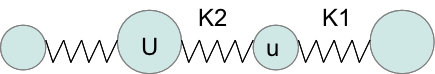
\includegraphics[scale=0.5]{diatomic.png}
\end{figure}
  \begin{itemize}
  \item Equations of Motion:
\begin{align*}
	M\frac{\partial ^2 u_n}{\partial t^2}&=-K1(U_n-u_n)-K2(U_n-u_{n-1})\\
	m\frac{\partial ^2 u_n}{\partial t^2}&=-K1(u_n-U_n)-K2(u_n-U_{n+1})
\end{align*}
 \item General solutions:
\begin{align*}
	U_n&=\sum_\kappa \tilde{U_\kappa}e^{i(\kappa n a-\omega t)} \hspace{10 mm}
	u_n=\sum_\kappa \tilde{u_\kappa}e^{i(\kappa n a-\omega t)}
\end{align*}
\end{itemize}
\end{frame}

\begin{frame}
  \frametitle{Diatomic Chain}   % Insert frame title between curly braces

  \begin{itemize}
 \item Eigenvalue problem representation:
\[
\begin{bmatrix}
  -M\omega_\kappa^2 & 0\\
  0 & -m\omega_\kappa^2\\ 
 \end{bmatrix}
\begin{bmatrix}
\tilde{U_\kappa} \\ 
\tilde{u_\kappa}
\end{bmatrix}
=
\begin{bmatrix}
  -(K1+K2) & K1+K2e^{-i\kappa a}\\
  -(K1+K2) & K1+K2e^{-i\kappa a}\\ 
 \end{bmatrix}
\begin{bmatrix}
\tilde{U_\kappa} \\ \tilde{U_\kappa}
\end{bmatrix}
\]
\item General version:
  \begin{align*}
	\omega^2(\kappa,\nu) e(\kappa,\nu)=D(\kappa)e(\kappa,\nu) 
  \end{align*}
\item The spring constant is determined by a material specific empirical potential
\end{itemize}
\end{frame} 

\begin{frame}
  \frametitle{Simple Phonon Properties}   % Insert frame title between curly braces

  \begin{itemize}
  \item Group Velocity:
\begin{align*}
v_g(\pmb{\kappa}, \nu)=\frac{\partial \omega(\pmb{\kappa},\nu)}{\partial \pmb{\kappa}}
\end{align*}
  \item Specific Heat:
\begin{align*}
c_{ph}(\pmb{\kappa},\nu)=\frac{\partial E}{V\partial T}=\frac{\hbar\omega(\pmb{\kappa},\nu)}{V}\frac{\partial f^{BE}(\pmb{\kappa}, \nu)}{\partial T}
\end{align*}
  \item We still need the phonon lifetimes $\tau(\pmb{\kappa}, \nu,L)$!
  \end{itemize}
\end{frame}

\begin{frame}
  \frametitle{What exactly is $\tau$}   % Insert frame title between curly braces

  \begin{itemize}
  \item Matthiesen rule:
\begin{align*}
\frac{1}{\tau(\pmb{\kappa}, \nu,L)}=\frac{1}{\tau_{p-p}(\pmb{\kappa}, \nu)}+\frac{1}{\tau_{b}(\pmb{\kappa}, \nu,L)}+\frac{1}{\tau_{p-e}(\pmb{\kappa},\nu)}
\end{align*}
  \item Boundary Scattering:
\begin{align*}
\tau_{b}(\pmb{\kappa}, \nu,L)=\frac{L/2}{|v_g(\pmb{\kappa}, \nu)|}
\end{align*}
  \item Electron-Phonon Scattering (low doping levels):
\begin{align*}
\frac{1}{\tau_{p-e}}=\frac{n_e\epsilon_1^2\omega}{\rho V_g^2k_BT}\sqrt{\frac{\pi m^{*}V_g^2}{2k_BT}}exp(-\frac{m^{*}V_g^2}{2k_BT})
\end{align*}
  \item How can we find $\tau_{p-p}$ numerically? Go beyond the harmonic approximation!
  \end{itemize}
\end{frame}

\begin{frame}
  \frametitle{Anharmonicity}   % Insert frame title between curly braces
  \begin{itemize}
  \item Selection Rules:
  \begin{align*}
	\hbar\omega(\pmb{\kappa},\nu)+\hbar\omega(\pmb{\kappa}',\nu')&=\hbar\omega(\pmb{\kappa}'',\nu'')\\
	\pmb{\kappa}+\pmb{\kappa'}=\pmb{\kappa''}+\pmb{g}
\end{align*}
  %\item	Harmonic Energy:
  %\begin{align*}
%	E=\frac{1}{2}\sum_n[G(U_n-u_n)^2+g(u_{n-1}-U_n)^2]
 % \end{align*}
  \item Thermal expansion and Finite Thermal conductivity:
  \begin{align*}
	E=N\phi+\sum_{s\geq1}\frac{1}{s!}\frac{\partial^s\phi}{\partial u^s}\sum_n(u_n-u_{n+1})^s
  \end{align*}
  \item Fermi's golden rule (empirical potentials are inadequate):
\begin{align*}
	\tau_{p-p}(\pmb{\kappa}, \nu) \propto \frac{\partial^3\phi(\pmb{\kappa}, \pmb{\kappa}',\pmb{\kappa}'')}{\partial u(\pmb{\kappa})\partial u(\pmb{\kappa}')\partial u(\pmb{\kappa}'')}
  \end{align*}
  \end{itemize}
\end{frame}

\begin{frame}
  \frametitle{Density Functional Theory}   % Insert frame title between curly braces
  \begin{itemize}
  \item Theorem 1: The ground-state energy from Schrodinger's equation is a unique function of the electron density.
  \item Theorem 2: The electron density that minimizes the energy of the overall functional is the true electron density corresponding to the full solution of the Schrodinger equation.
  \item The Kohn-Sham single electron equations have the form:
\begin{align*}
	[\frac{\hbar^2}{2m}\nabla^2+V(\vec{r})+V_H(\vec{r})+V_{XC}]\psi_i(\vec{r})=\epsilon_i\psi_i(\vec{r})
\end{align*}
  \end{itemize}
\end{frame}

%\begin{frame}
%  \frametitle{Adiabatic Approximation}   % Insert frame title between curly braces

% \begin{itemize}
%  \item Born Approximation:
%The nuclear and electronic degrees of freedom become decoupled. 
%The electrons are hereby assumed to follow the motion of the atomic core without exchanging energy with its surroundings.
%  \end{itemize}
%\end{frame}

\begin{frame}
  \frametitle{Iteration procedure in DFT}   % Insert frame title between curly braces
  \begin{itemize}
  \item A trial electron density is chosen: $n_1(r)$
  \item Solve Kohn-Sham with initial guess: 
\begin{align*} 
[\frac{\hbar^2}{2m}\nabla^2+V(\vec{r})+e^2\int\frac{n_1(\vec{r'})}{|\vec{r}-\vec{r'}|}d^3\vec{r'}+V_{XC}^{electron gas}[n_1(\vec{r})]]\psi_i(\vec{r})=\epsilon_i\psi_i(\vec{r})
\end{align*}
  \item Recaculate electron density:
 \begin{align*} 
	n_2(\vec{r})&=2\sum_i\psi_i^*(\vec{r})\psi_i(\vec{r})
	    \end{align*}
  \item Iterate until $n_{p+1}(\vec{r})=n_{p}(\vec{r})$	
  \end{itemize}
\end{frame}

\section{Results}
\begin{frame}
  \frametitle{Bulk Silicon from DFT}   % Insert frame title between curly braces

\begin{figure}[ht]
\centering
\subfigure[Dipersion]{
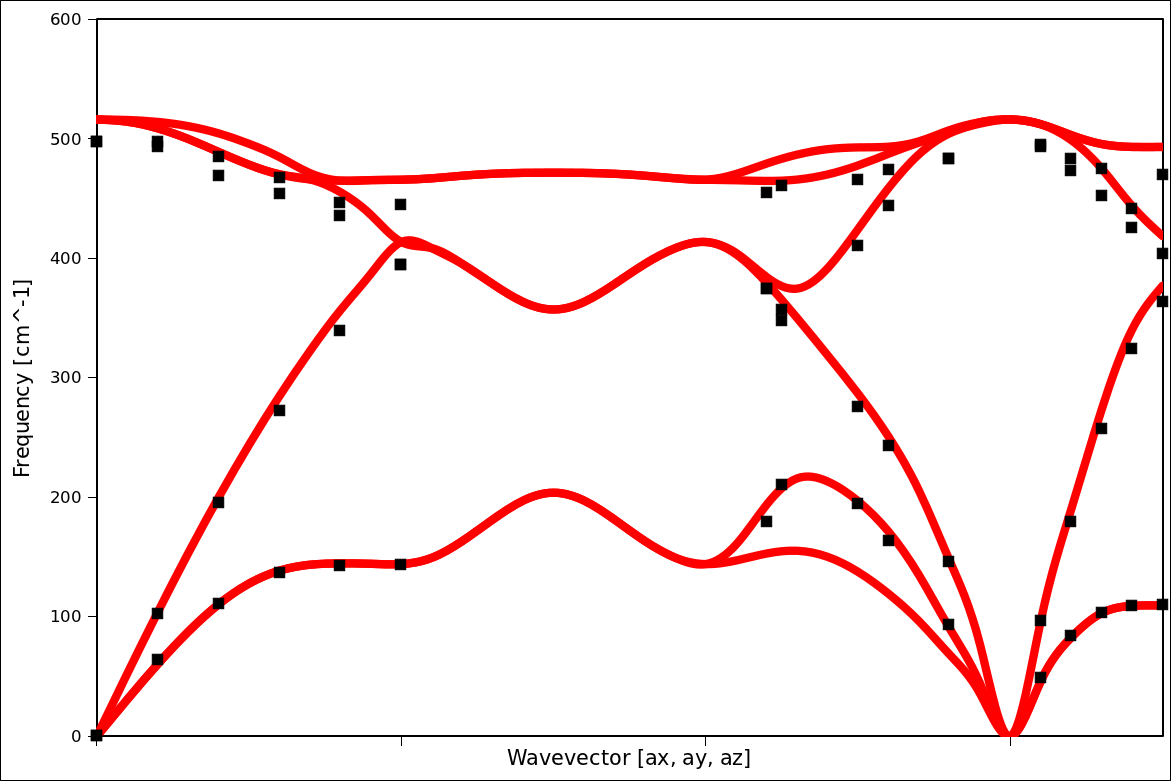
\includegraphics[scale=0.12]{dispersion1.png}
\label{fig:subfig1}
}
\subfigure[Density of States]{
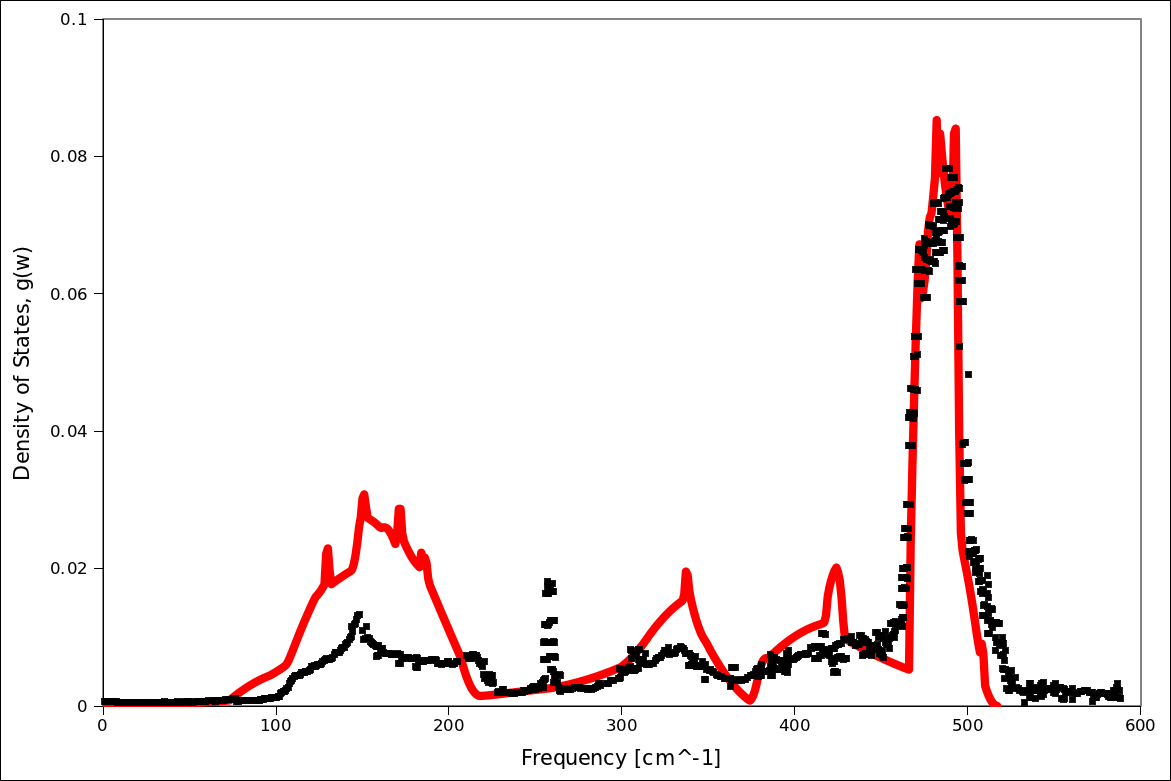
\includegraphics[scale=0.12]{dos1.png}
\label{fig:subfig2}
}
\end{figure}
 
\end{frame}

\begin{frame}
  \frametitle{Silicon cont.}   % Insert frame title between curly braces
\begin{itemize}
  \item Lifetimes????
 \end{itemize}
\end{frame}

\section{Conclusions}

\begin{frame}
  \frametitle{So What Just Happened?}   % Insert frame title between curly braces
 \begin{itemize}
  \item DFT for bulk phonon properties
  \item Lifetimes are not any easy task
  \item Extend this approach to the nanoscale
 \end{itemize}
\end{frame}

\note{The end}       % Add notes to yourself that will be displayed when
		     % typeset with the notes or notesonly class options


\end{document}
